% !BIB program=biber
\documentclass[scheme=chinese,a4paper]{article}
\usepackage[utf8]{inputenc}
\usepackage{amsmath}
\usepackage{esint}
\usepackage{tabstackengine}
\usepackage{xeCJK}
\usepackage{caption}
\usepackage{stackengine}
\usepackage{graphicx}
\graphicspath{ {./figure/} }
\usepackage{float}
\usepackage{amsmath}
\usepackage{ulem}
\usepackage{amsfonts}
\usepackage{xcolor}
\usepackage{tikz}
\usetikzlibrary{calc}
\usepackage{pgfplots}
\usepackage{mathrsfs}
\usepackage{listings}
\lstset{basicstyle=\ttfamily\footnotesize,breaklines=true}
\usepackage{url}
\usepackage[colorlinks,linkcolor=black]{hyperref}
\usepackage{enumitem}
\setlist[1]{itemsep=-5pt}
\usepackage{subcaption}
\usepackage{pdfpages}
\usepackage{booktabs}
\usepackage{multirow}
\usepackage[toc,page]{appendix}


\usepackage[backend=biber,style=gb7714-2015]{biblatex} 
\addbibresource{../resources/bibs/refs.bib}

\usetikzlibrary{shapes,arrows}
\usetikzlibrary{arrows}

%%%% 下面的命令重定义页面边距,使其符合中文刊物习惯 %%%%
\addtolength{\topmargin}{-54pt}
\setlength{\oddsidemargin}{0.63cm}  % 3.17cm - 1 inch
\setlength{\evensidemargin}{\oddsidemargin}
\setlength{\textwidth}{14.66cm}
\setlength{\textheight}{24.00cm}    % 24.62

%%%% 段落首行缩进两个字 %%%%
\makeatletter
\let\@afterindentfalse\@afterindenttrue
\@afterindenttrue
\makeatother
\setlength{\parindent}{2em}  %中文缩进两个汉字位

%%%% 下面的命令设置行间距与段落间距 %%%%
\linespread{1.4}
% \setlength{\parskip}{1ex}
\setlength{\parskip}{0.5\baselineskip}

%%%% 重定义 %%%%
\renewcommand{\contentsname}{目录}  % 将Contents改为目录
\renewcommand{\abstractname}{摘要}  % 将Abstract改为摘要
\renewcommand{\refname}{参考文献}   % 将References改为参考文献
\renewcommand{\indexname}{索引}
\renewcommand{\figurename}{图}
\renewcommand{\tablename}{表}
\renewcommand{\appendixpagename }{附录}
\renewcommand{\appendixtocname }{附录}
% \renewcommand{\algorithm}{算法}

\title{Report}
\author{Crosstyan}
\date{Sep 2020}

\begin{document}
\begin{center}
    \tableofcontents\clearpage
\end{center}

% \begin{center}
%     \textbf{无线运动传感器节点设计}
% \end{center}
\begin{abstract}
本作品由ADS1292R模块,LMT70测温模块,MPU6050加速度计步检测模块,再结合Arduino和ESP32系列MCU和基于Node.js的服务器组成。

\textbf{关键词:}Node.js、物联网、心率检测
\end{abstract}

\section{方案综述}
\begin{figure}[H]
    \centering
    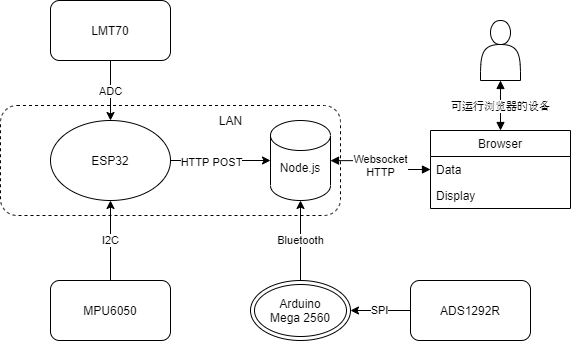
\includegraphics[width=1\textwidth]{figure.png}
    \caption{系统框图}
\end{figure}
根据题目要求可得到系统的总体框图,如图1所示。\par
人体产生的心电信号经过ADS1292R模块的处理后,产生含有少量噪声的心电信号,传输给Arduino Mega 2560板处理得到心率数据。
Arduino再通过蓝牙模块直接传送数据到Node.js服务器. 

与此同时MPU6050加速度计步检测模块通过对人体行进时$x,y,z$三轴加速度的变化计算得到人行进时的步数, 
并且LMT70芯片对空气中温度变化敏感,而引起的芯片输出电压的变化。
LMT70测温模块、MPU6050加速度检测模块与ESP32直接相连, 将收集到的数据进行处理后以JSON格式通过HTTP协议传输到本地服务器。
最后,Node.js服务器后端利用Websocket协议将数据处理后发送给前端页面显示。用户可以使用浏览器接收到所需的数据. 

ESP32、Arduino和执行Node.js的服务器终端必须要求在同一局域网之内,其中有多种类型的设备可以运行Node.js作为服务器, 如路由器, 树莓派等。本次作品采用笔记本电脑作为Node.js的服务器端设备进行操作. 

% \subsection{加速计模块的论证与选择}
% \textbf{方案一:}采用AXL345芯片设计的计步器通过对三个方向的加速度进行分析

% \textbf{方案二:}采用MPU6050芯片设计的计步器通过分别对x、y、z方向上的加速度采集数据,
% 采用波峰波谷检测的方法计算步数, 除了,算法比较简单,精度比方案一稍差,但是符合题目要求,且易于实现。因此采用方案二.




\section{理论分析与计算}
% 采用数字滤波器组法:它是由线性数字滤波、非线性变换和决策算法三个部分
% 组成。首先用一组数字滤波器滤除分析对象以外的信息、达到抑制噪声干扰的目
% 的,以便于提取出波特征的信息。通常的做法是采用带通滤波,提高
% 频率范围内信号的分量,使波群的能量得到加强。然后采用阈值判断、
% 斜率判断等方法对特征点进行判断,实现检测波的目的,并采取一些补偿策略
% 提高检测的准确度 。

\subsection{体表温度测量方法}
采用归一化加权平均算法,
每进行一次测量,对人体进行多次采样,得到温度的测量数列,
首先得到拥有一致性的测量数据,然后依据本算法得出融合值,
进而算出温度的准确测量结果,去除过程中的不确定性

    % \bar{X}&=\frac{1}{N}\sum_{i\in[1,N]}^mX_i\\
    % \Delta X_i&=X_i-\bar{X}\\
    % f(\Delta X_i)&=(\frac{1}{\pi*\Delta Xi})*\arctan(\frac{1}{\Delta Xi})\\
    % \bar{\Delta a_i}&=f(\Delta X_i) \\ 
    % \bar{a_i}&=\frac{\Delta \bar{a_i}}{\sum_{i\in[1,N]} \Delta \bar{a_i}}\\
    % X^+&=\sum_{i\in[1,N]}X_i*\bar{a_i}

 由一致性数组$X\in[1,N]$能够得出被测数据的平均值 
\begin{equation}
    \bar{X}=\frac{1}{N}\sum_{i\in[1,N]}^mX_i
\end{equation}
计算每一测量值$X_i$相对于均值$\bar{X}$的偏差量$\Delta X_i$
\begin{equation}
    \Delta X_i=X_i-\bar{X}
\end{equation}
权值函数
\begin{equation}
    f(\Delta X_i)=(\frac{1}{\pi*\Delta Xi})*\arctan(\frac{1}{\Delta Xi})  
\end{equation}
 将偏差量$\Delta X_i$代入权值函数 $f(X)$,作归一化处理 $\bar{\Delta a_i}$
\begin{equation}
    \bar{\Delta a_i}=f(\Delta X_i)
\end{equation}
由归一化偏差量得到加权值$\bar{a_i}$
\begin{equation}
    \bar{a_i}=\frac{\Delta \bar{a_i}}{\sum_{i\in[1,N]} \Delta \bar{a_i}}
\end{equation}
由加权值得到最终的平均值$X^+$
\begin{equation}
    X^+=\sum_{i\in[1,N]}X_i\times\bar{a_i}
\end{equation}
\subsection{LMT70温度算法}
查LMT70的数据表易知, 可以使用一阶传递函数来计算LMT70所感测的温度,但是在较宽的温度范围内,它是最不准确的方法。我们使用在电气特性温度查找表(LUT)中找到的LUT(查找表)信息可以轻松生成方程式。其二阶传递函数为
\begin{equation}
  T_M=a\cdot(V_{\text{TAO}})^2+b\cdot(V_{\text{TAO}})+c
\end{equation}
更加精确的三阶传递函数为
\begin{equation}
  T_M=a\cdot(V_{\text{TAO}})^3+b\cdot(V_{\text{TAO}})^2+c\cdot V_{\text{TAO}}+c
\end{equation}
\subsection{运动量统计}
采用波峰波谷检测法。人体迈步过程中,重心会随着人体运动在一定范围内出现规律性的变化。
脚蹬地离开地面时,地面的反作用力会使垂直加速度开始增大,身体重心上移,
当脚达到最高位置时,脚的垂直速度最小,但垂直加速度最大。当脚向下落时,
垂直加速度开始减小,落地时加速度达到最小值。在运动过程中,
加速度传感器会根据人体运动的频率采集到$x,y,z$三轴的加速度数值,形成一个波形图。
在波形图中存在波峰和波谷,检测步数其实就是检测波峰。
行走时,由加速度传感器获取的数值经过检测如果为波峰,
并且两次波峰的时间以及阈值符合设定的数值范围,那么即可算作用户走了一步,
超过这个设定的范围则看作用户停止步行或者无效行走。
\begin{figure}[H]
    \centering
    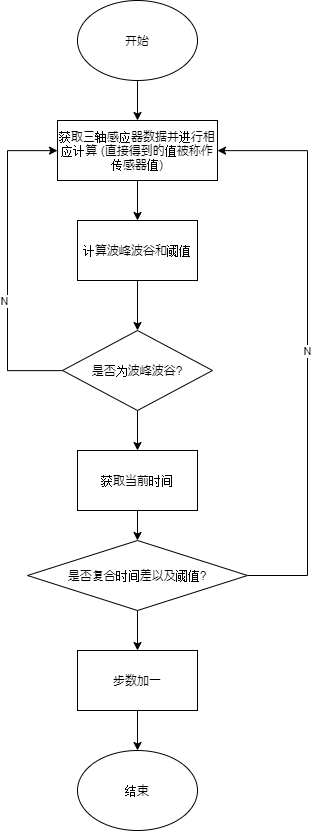
\includegraphics[width=0.3\textwidth]{algritom.png}
    \caption{算法流程图}
\end{figure}

%$$\alpha_{\theta}=\iint_{S}\vec{A} d\theta$$
%\begin{figure}[H]
%\centering
%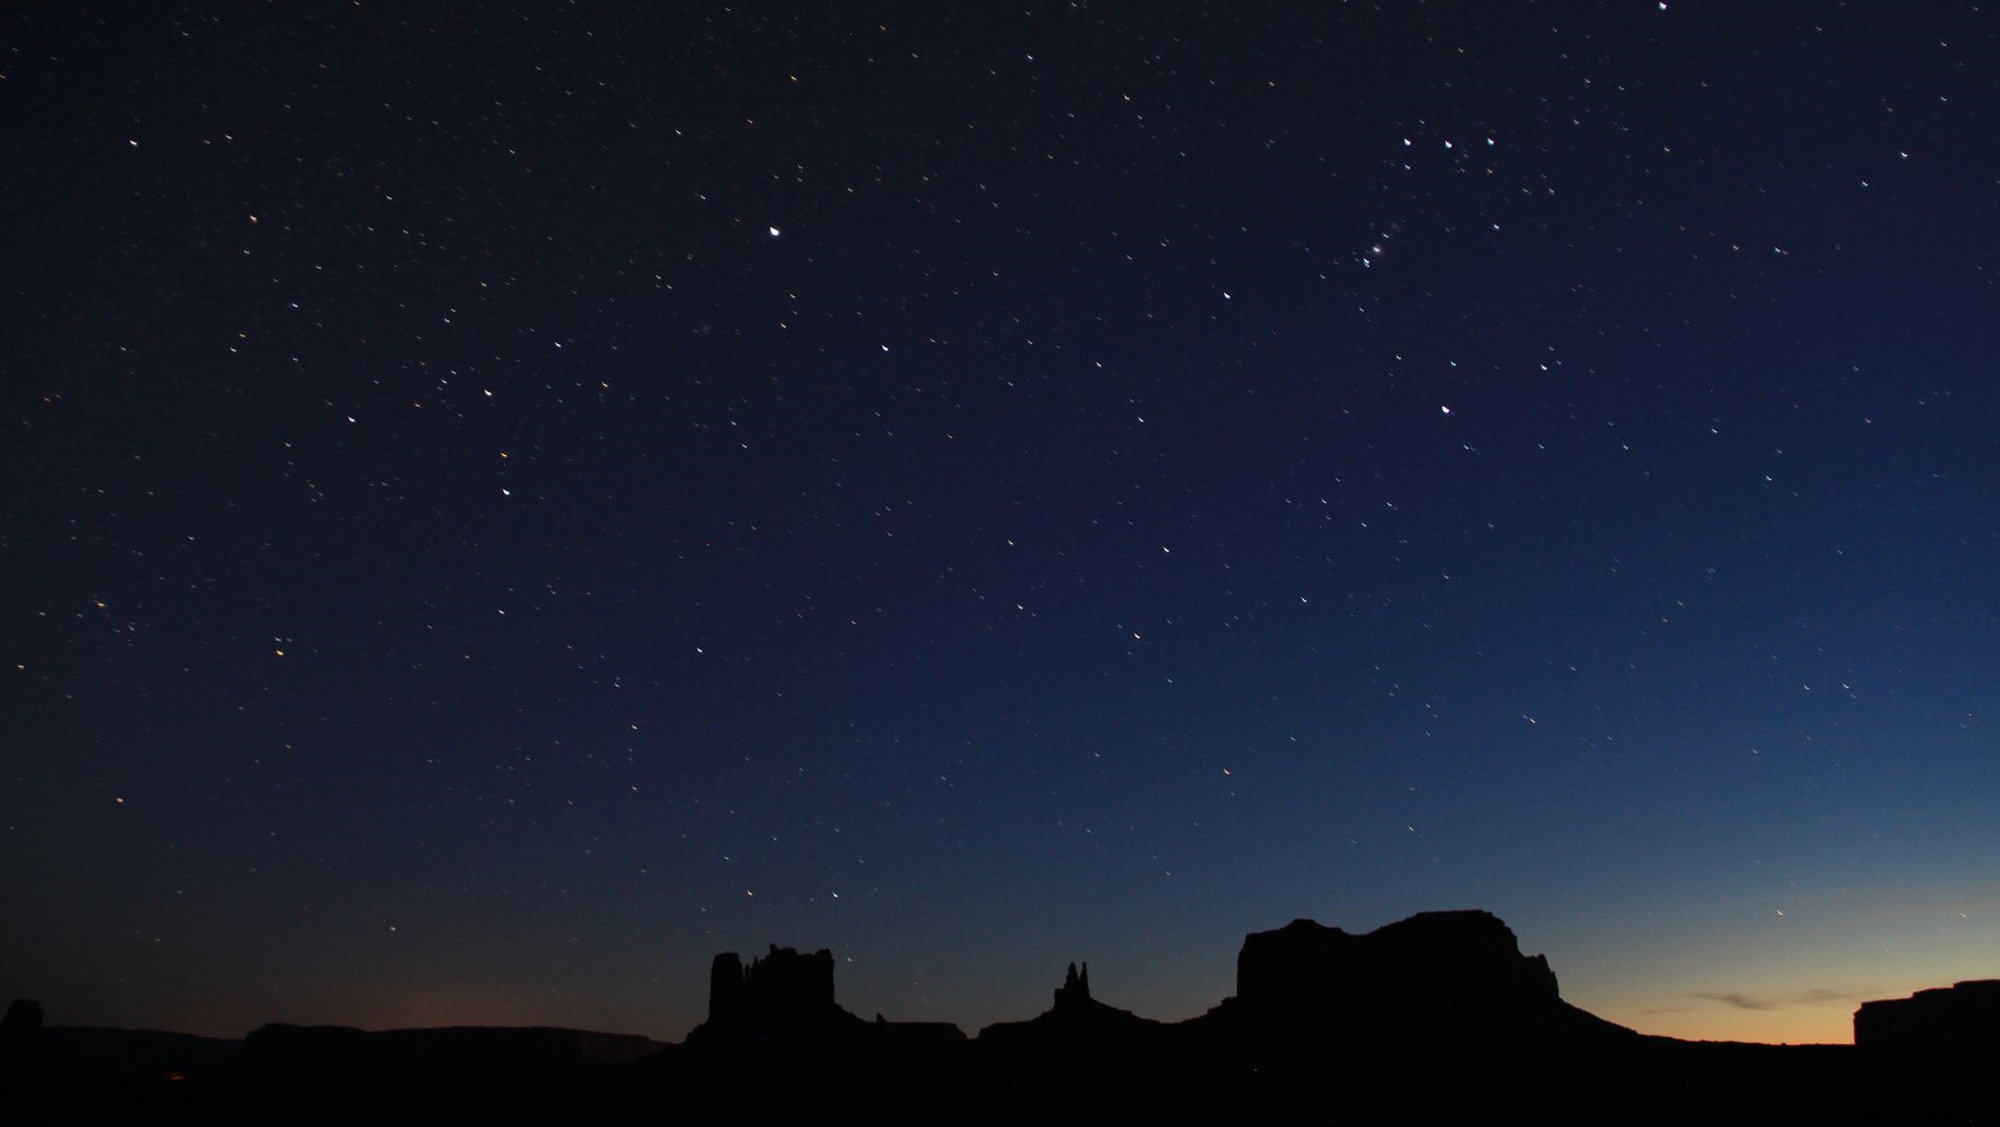
\includegraphics[width=0.33\textwidth]{1.png}
%\caption{night sky}
%\end{figure}
% \section{电路设计}
% \begin{figure}[H] %添加剩余模块的电路图
%     \centering
%     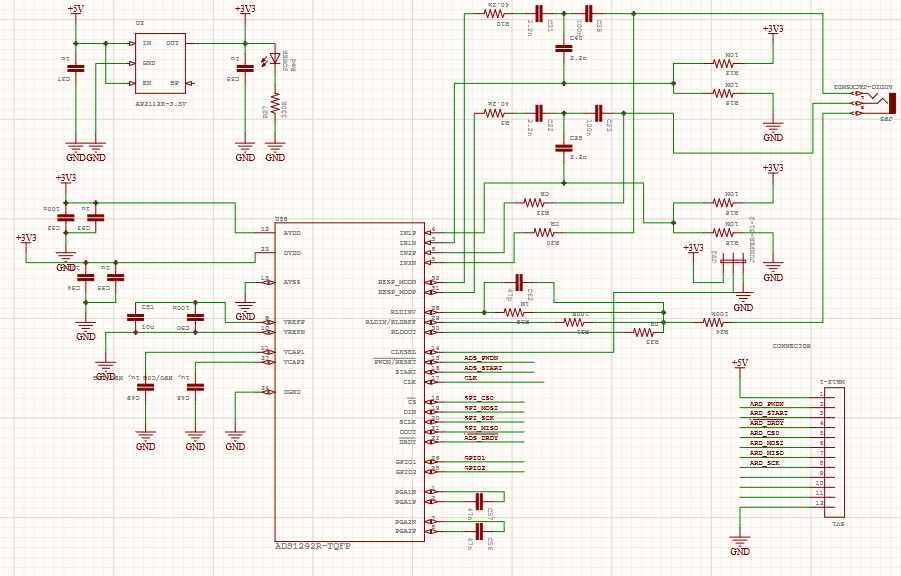
\includegraphics[width=0.8\textwidth]{ADS1292R心电产生模块.png}
%     \caption{心电测量模块电路图}
% \end{figure}
\section{各模块简介}

\subsection{Arduino心电数据数据处理层}
ADS1292的数据会经过Arduino的外接的HC-05蓝牙模块与Node.js服务器进行沟通. Arduino是一款便捷灵活、方便上手的开源硬件产品,其标准化的接口模式为它的可持续发展奠定了坚实的基础。
\subsection{ESP32}
ESP32带有蓝牙与WiFi模块,这意味着你可以通过Wi-Fi或蓝牙以极低的价格轻松地远程控制和监控设备。但由于其GPIO引脚口数目有限, 使得其无法直接接入ADS1292模块. 但是ESP32可以方便的采集处理以及传输来自LMT70和MPU6050的数据. 
% \textbf{方案一:}
% 使用PHP。PHP是一种开源的通用计算机脚本语言,尤其适用于网络开发并可嵌入HTML中使用。
% PHP诞生较早,所以在文档,API和代码库等在线资源方面更为丰富,但是符合我们开发需求的资源较少。

% \textbf{方案二:}
\subsection{后端服务器层}
使用Node.js和HTTP协议作为服务器层的处理架构. 之所以使用HTTP而非MQTT作为沟通协议是因为其以TCP为传输层的特点, 保证了数据的完整发送和接收.  其易于操作与实现, 且在各个终端设备均可使用, 不局限于移动端或者桌面端. 

Node.js是一个Javascript运行环境。Node.js 使用事件驱动,非阻塞I/O 模型而得以轻量和高效. 当Node.js 执行I/O 操作时(例如从网络读取、访问数据库或文件系统),  Node.js会在响应返回时恢复操作,而不是阻塞线程并浪费CPU 循环等待。非常适合于处理大量终端设备连接时的情形. 其强大的扩展功能亦保证了蓝牙模块的正确接入. 
\subsection{前后端沟通层}
WebSocket的诞生本质上就是为了解决HTTP协议本身的单向性问题:请求必须由客户端向服务端发起,然后服务端进行响应。比起传统的Ajax来说更为简练明了. 
\subsection{前端显示层}
\begin{figure}[H]
\centering
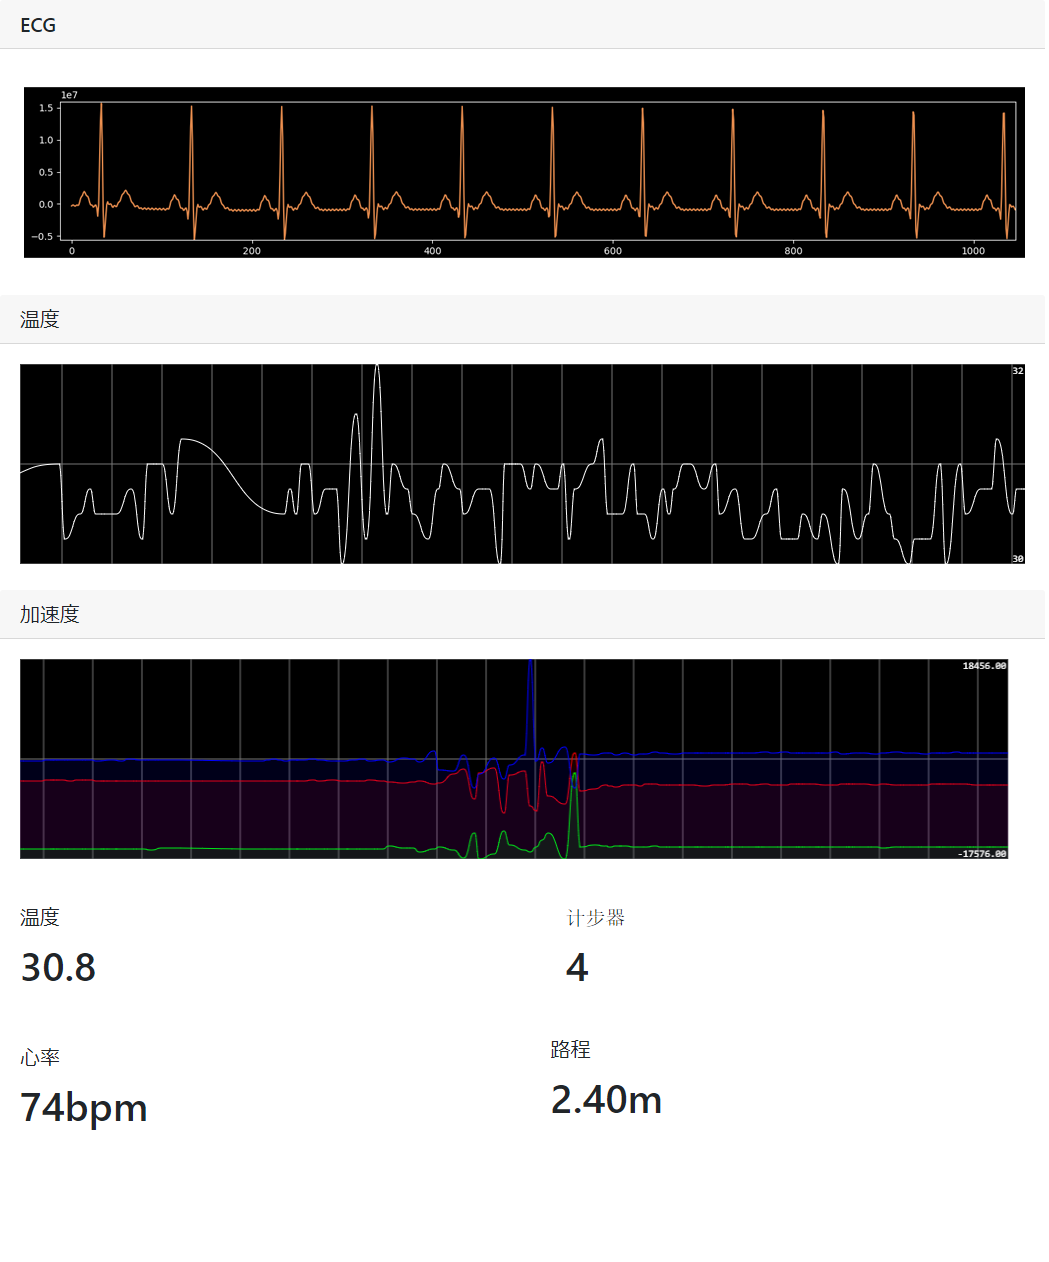
\includegraphics[width=0.5\textwidth]{final.png}
\caption{前端页面测试效果}
\end{figure}
因为Web只需要页面开发,没有开发语言的限制也没有客户端和服务端的限制问题,这样就会使成本大大降低。Web是可以跨平台的,这样就节省了下载安装的时间,也不会占用手机内存和手机流量。同时也有很好的展示效果. 
% \section{测试方案与结果}
% Table generated by Excel2LaTeX from sheet 'Sheet1'
\begin{appendices}
\section{测试数据}
\subsection{心率测试}
\begin{table}[H]
  \centering
    \begin{tabular}{ccc}
    \toprule
    \multirow{2}[2]{*}{芯片测得的心率} & \multirow{2}[2]{*}{手环测得的心率} & \multirow{2}[2]{*}{误差} \\
          &       &  \\
    \midrule
    87    & 88    & 1.15\% \\
    \midrule
    86    & 88    & 2.33\% \\
    \midrule
    87    & 87    & 0.00\% \\
    \bottomrule
    \end{tabular}%
  \caption{心率测试精度统计}
  \label{tab:addlabel}%
\end{table}%


% Table generated by Excel2LaTeX from sheet 'Sheet1'
\subsection{温度测试}
% Table generated by Excel2LaTeX from sheet 'Sheet1'
% Table generated by Excel2LaTeX from sheet 'Sheet1'
\begin{table}[H]
  \centering
    \begin{tabular}{cccc}
    \toprule
    \multirow{2}[2]{*}{芯片测得的温度} & \multirow{2}[2]{*}{测温枪测得的温度} & \multirow{2}[2]{*}{误差度数} & \multirow{2}[2]{*}{误差} \\
          &       &       &  \\
    \midrule
    35.00  & 34.40  & 0.6   & 1.71\% \\
    \midrule
    34.70  & 35.00  & 0.3   & 0.86\% \\
    \midrule
    34.80  & 34.60  & 0.2   & 0.57\% \\
    \bottomrule
    \end{tabular}%
  \caption{温度测量统计}
  \label{tab:addlabel}%
\end{table}%



\subsection{运动统计测试}
% Table generated by Excel2LaTeX from sheet 'Sheet1'
\begin{table}[H]
  \centering
    \begin{tabular}{ccc}
    \toprule
    \multirow{2}[2]{*}{芯片测得的步数} & \multirow{2}[2]{*}{手环测得的步数} & \multirow{2}[2]{*}{误差} \\
          &       &  \\
    \midrule
    10.00  & 14.00  & 0.00\% \\
    \midrule
    15.00  & 16.00  & 6.67\% \\
    \midrule
    30.00  & 31.00  & 3.33\% \\
    \bottomrule
    \end{tabular}%
  \caption{计步器功能统计}
  \label{tab:addlabel}%
\end{table}%
\end{appendices}
\end{document}